\chapter{Background} % nothing of mine

% utrolig mye bra her: https://www.dei.unipd.it/\~emg/downloads/SIMPAR08-WorkshopProceedings/TeachingWithRobotics/karatrantou.pdf!! veldig mange bra kilder

% og mange eksempler herfra: https://student.cs.uwaterloo.ca/~cs231/resources/pseudocode.pdf

% mer på pseudokode: https://www.researchgate.net/profile/Nicholas-Bennett-6/publication/309410533\_Introduction\_to\_Algorithms\_and\_Pseudocode/links/60a489d04585158ca05c54bc/Introduction-to-Algorithms-and-Pseudocode.pdf

% Bra språk for å snakke om flowcharts: https://www.researchgate.net/publication/234805404_Flowchart_techniques_for_structured_programming

This chapter will cover key concepts one should be familiar with in order to fully understand the rest of this thesis. We start by providing a definition for pseudocode, before we discuss Haskell as an implementation language. Lastly, we discuss transpiling, and how some existing transpilers work.

\section{Pseudocode}

Pseudocode is a technique for describing computer programs in a more abstract way than programming languages allow, void of a predefined set of rules. Authors can ignore specific syntax and keywords, and instead put their focus on getting their ideas across. This can make programs easier to understand for both non-programmers and programmers alike, particularly when working with unfamiliar algorithms~\cite{whatIsPseudocode}. \\

Since it does not follow any precise syntax rules, pseudocode is subsequently not executable. This is not a bug, but rather a feature of pseudocode: it is intended for \textit{presenting ideas} of code, not \textit{demonstrating results} of code. As Donald Knuth famously put it, after presenting some algorithm implementations in pseudocode~\cite{famousKnuthQuote}:

\begin{verbatim}
    Beware of bugs in the above code; I have only proved
    it correct, not tried it.
\end{verbatim}

% As such, pseudocode is an abstract concept, and can technically be anything, as long as it aims to aid others in understanding what a particular piece of code does. \\

When explaining a solution to a non-technical audience, it makes more sense to use pseudocode than source code. More specifically, pseudocode that encapsulates the program's core functionality, to provide clarity on its essential aspects. This enables even individuals without a programming background to provide feedback, based on their understanding of both the problem and now also the proposed solution. \\

Now, since pseudocode has many faces, we must define what we really mean when we refer to pseudocode in the coming sections. In the context of this thesis, we believe that pseudocode can work as an umbrella term for both traditional pseudocode flowcharts.

\subsection{Traditional Pseudocode}

The most conventional form of pseudocode, commonly found in text books on algorithms, published papers, as well as design documents discussing problems~\cite{pseudocodeInBook1, pseudocodeInBook2, pseudocodeInPaper1, pseudocodeInPaper2}. It is also the form that most closely resembles source code, given that it usually includes line numbers, assign statements, and generally presents the problem solution in an imperative matter~\cite[247]{pseudocodeTendsToBeImperative}. \\

\forsup{Angående siste kilde: Det er side 2 i PDFen (\url{https://dl.acm.org/doi/pdf/10.1145/65294.71222}), men sidetallet på selve dokumentet viser 247. Er det da riktig å referere til side 247 eller 2?}

Since there is no formal set of rules commanding how pseudocode should look, we are prone to viewing different variations of the same algorithms across different literatures. A frequently presented algorithm is \textbf{Binary search}, a search algorithm that finds the position of a target value within a sorted array. If the target value is not found, some sort of default value is usually returned~\cite{pseudocodeInBook1}. \\

In a note made for the Algorithmic Problem Solving course at the University of Waterloo, professor Naomi Nishimura presented four different variants of the Binary Search algorithm, all written in pseudocode~\cite{differentVersionsOfBinarySearch}. The algorithms are written with a total interval of 26 years from the oldest to the newest. \\

The oldest variant is from 1974, presented in The Design and Analysis of Computer Algorithms by Aho et al.~\cite[139]{binarySearchSource1}. Roughly 17 years later, Lewis et al. present their own version in Data Structures and Their Algorithms~\cite[182]{binarySearchSource2}. The underlying logic stays much the same, though the approaches and syntaxes are different, as seen in \Cref{Binary Search by Aho et al.} and \Cref{Binary Search by Lewis et al.}, respectively. \\

\begin{lstlisting}[caption={Binary Search by Aho et al.}, captionpos=b, label={Binary Search by Aho et al.}]
procedure SEARCH(a, f, l):
if f $>$ l then return "no"
else
    if a = A[$\lfloor$(f + l)/2$\rfloor$] then return "yes"
    else
        if a < A[$\lfloor$(f + l)/2$\rfloor$] then
            return SEARCH(a, f, $\lfloor$(f + l)/2$\rfloor$ - 1)
        else return SEARCH(a, $\lfloor$(f + l)/2$\rfloor$ + 1, l)
\end{lstlisting}

\begin{lstlisting}[basicstyle=\footnotesize\ttfamily, caption={Binary Search by Lewis et al.}, captionpos=b, label={Binary Search by Lewis et al.}]
function BinarySearchLookUp(key K, table T[0..n-1]): info
{Return information stored with key K in T, or $\Lambda$ if K is not in T}
    Left $\gets$ 0
    Right $\gets$ n - 1
    repeat forever
        if Right < Left then
            return $\Lambda$
        else
            Middle $\gets$ $\lfloor$(Left + Right) / 2$\rfloor$
            if K = Key(T[Middle]) then return Info(T[Middle])
            else if K < Key(T[Middle]) then Right $\gets$ Middle - 1
            else Left $\gets$ Middle + 1
\end{lstlisting}

The wish for automatic generation of pseudocode has been desired for some time, with the intention of presenting ideas without having to worry about the syntax of a particular programming language~\cite{desireToGetPseudocodeGeneration}. Traditional pseudocode allows us to draft ideas in an imperative fashion, the same way we write baking recipes and instructions for building legos. Here, the author is free to omit boilerplate code, include mathematical notation and necessary abstractions, and even resort to natural language where deemed appropriate~\cite{pseudocodeInBook1, freedomOfPseudocode}. \\

As previously mentioned, pseudocode has a well-established history in university curricula. When learning algorithms, data structures, and programming concepts in general, the focus is really on the underlying ideas. The concepts are generally more important than the specifics of how they are implemented in a particular programming language. Thus, the approach of learning with pseudocode prioritises concept comprehension over language-specific knowledge. \\

The usefulness of having a tool translating source code to pseudocode can also be backed by a number of factors. For one, there exists several online translators like PseudoEditor and Code Kindle.~\footnote{A DSL that can be found at \url{https://pseudoeditor.com/}.}~\footnote{Works with C++ and Python, can be found at \url{https://devpost.com/software/code-kindle}. Its source code is also available at \url{https://github.com/Open-Sourced-Olaf/Code-Kindle}.} There has also been a fair share of research going into the topic, most notably by Oda et al. and Alhefdhi et al.~\cite{pseudogen, pseudocodeGenerator}. Lastly, there are still being created new styles for dislaying pseudocode~\cite{displayingPseudocode}.

% There are several software available for translating source code to pseudocode, The latter utilises statistical machine translation for the translation part, and works with both C++ and Python.~\footnote{SMT is a technique to train a model on previously translated and analyzed information and conversations. It is commonly used to translate between natural languages.} In 2015, Oda et. al introduced Pseudogen~\cite{pseudogen}, which also uses statistical machine translation, and works with Python. The tools that employ statistical machine translation both translate their source programs entirely to natural language. \\

\subsection{Flowcharts}

Not all programming languages share the same execution flow. For instance, all processes in a VHDL description are executed concurrently~\cite{vhdl}. In languages with term rewriting, like Maude~\cite{maude}, rewriting rules are applied non-deterministically --- if multiple rules can apply to a term, any one of them may be chosen in an arbitrary order. \\

Some languages, on the other hand, like Python, will execute their programs line for line. This means that we can almost follow the execution flow by just looking at the order functions are called, and the order of statements within those functions. \\

This way of executing a program opens up for the possibility of converting source code to flowcharts, which still includes text, but also complements it with shapes, arrows and colours. When code stretches over enough lines, it often becomes uniform in appearance and more challenging to comprehend. By contrast, flowcharts explicitly capture the control flow of the program, and makes it possible to direct our focus. \\

Images in computer science is nothing new. One of the most notable examples we have are the ones we use for finite state automata (FSA). An FSA is a machine which either accepts or rejects a given string, by running each symbol through a state sequence uniquely determined by said string. We differentiate betwee deterministic and non-deterministic FSAs, although that is not of importance in our context. What they share, is a number of states, a start state, a transition function and an accept state~\cite{introToAutomataTheory}. \\

\begin{figure}[ht]
    \centering
    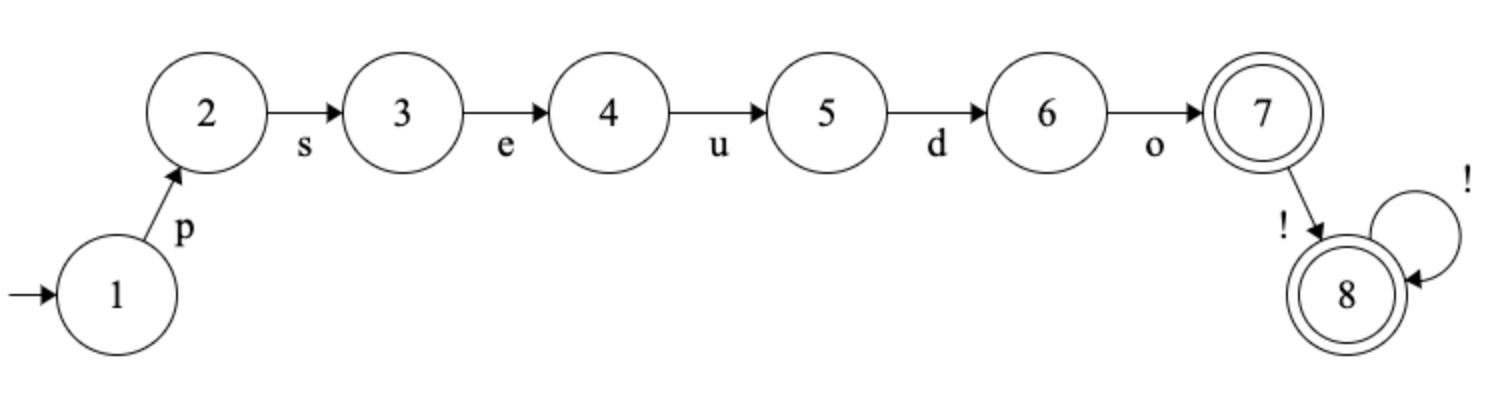
\includegraphics[scale=0.46]{assets/dfa.png}
    \caption{A finite state automata.}
    \label{An example finite state automata.}
\end{figure}

\Cref{An example finite state automata.} shows an example of an FSA which accepts the word \textbf{pseudo} followed by an arbitrary number of exclamation marks. The FSA has 8 states, and the leftmost arrow indicates that \textbf{1} is the starting state. From here, we can get to the second state if our string starts with the symbol \textbf{p}. Thus, all strings that do not begin with a \textbf{p} are rejected at this point. States 7 and 8 have an additional ring within their circle, which means that they are accepting states. If a combination of symbols have not been rejected at this point, and is finished, it is accepted. \\

State 8 has an arrow leading to itself via the symbol \textbf{!}, meaning that it can end with as many exclamation marks as possible. A string like \textbf{pseudo!!p!!!} is not accepted, however, despite starting with \textbf{pseudo!!} and ending with \textbf{!!!}. Once a string has reached state 8, it can \textit{only} be followed by exclamation marks, or else it is rejected. \\

Warren McCulloch and Walter Pitts were among the first researchers to introduce a concept similar to finite automata, all the way back in 1943~\cite{firstFSA}. Their paper presents a simplified computational model of biological neurons. \\

There have been multiple attempts to create flowchart editors, most notably by Carlisle et al. and Charntaweekhun et al.~\cite{flowchartEditor1, flowchartEditor2}. These allow us to build flowcharts using the drag-and-drop approach, rather than keeping it all in text form. Benefits of learning with help from visual aid is well documented, and when it comes to computer science, visualisations are especially prominent in the context of machine learning~\cite{ML_Visual1, ML_Visual2, ML_Visual3}. \\

One of few editors that generates flowcharts directly from code is Code2Flow\footnote{Can be found at \url{https://app.code2flow.com/}}. This is a DSL with support for most common programming concepts like statements, loops, conditionals, and more. The editor comes with a comprehensible guide on its syntax. It is also a highly customisable tool: it lets us change the flowcharts' fonts, colours, sizes and even edge height. \Cref{Code2Flow source code and flowchart} shows a side-by-side comparison of a simple program written with Code2Flow and its corresponding flowchart. \\

\begin{figure}[ht]
\centering
    \begin{subfigure}{.5\textwidth}
      \centering
      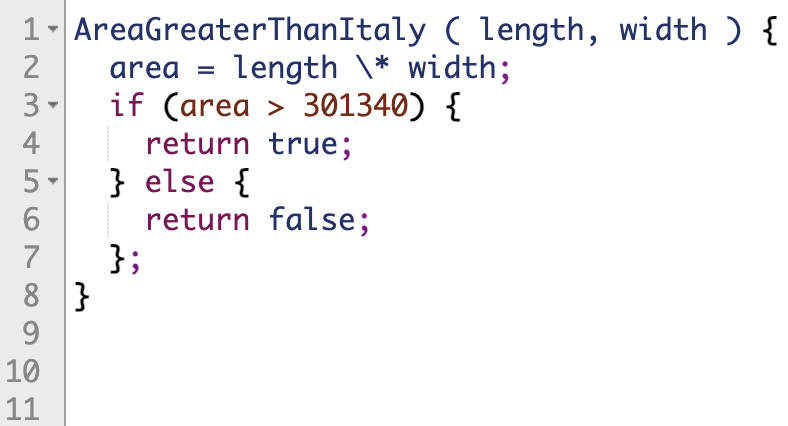
\includegraphics[width=1\linewidth]{assets/c2f_c.png}
      \caption{Screenshot of a program written in Code2Flow source code.}
      \label{Code2Flow source code}
    \end{subfigure}
    \begin{subfigure}{.3\textwidth}
      \centering
      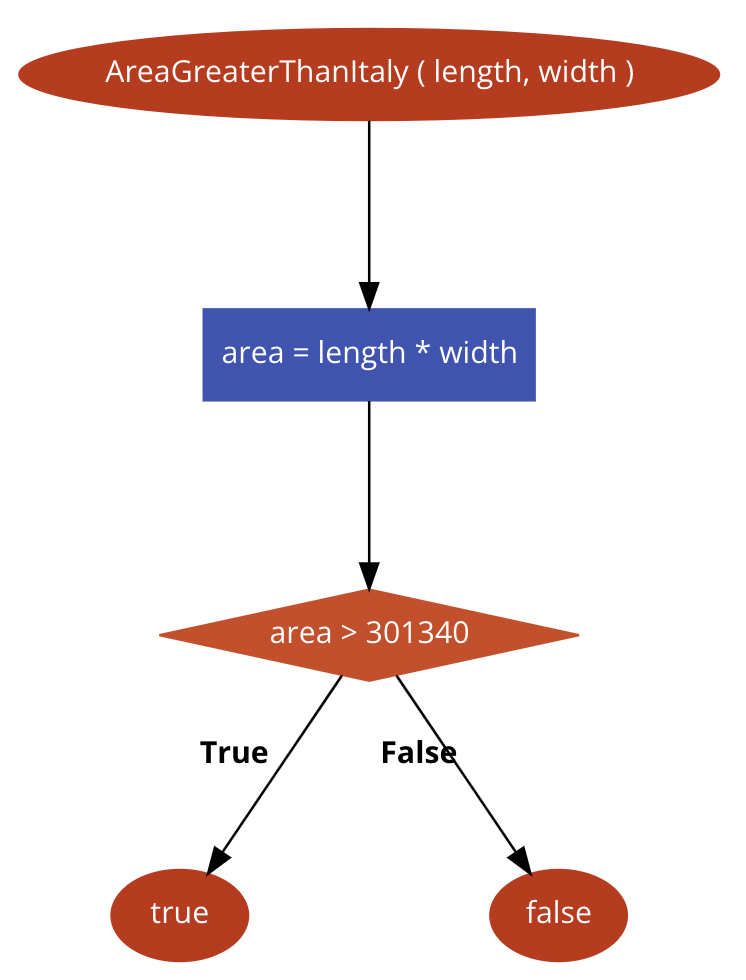
\includegraphics[width=1\linewidth]{assets/c2f_r.png}
      \caption{The compiled result of \Cref{Code2Flow source code}.}
      \label{Compiled Code2Flow result}
    \end{subfigure}

\caption{An algorithm written with Code2Flow, and the corresponding flowchart.}
\label{Code2Flow source code and flowchart}
\end{figure}

Given the imperative nature of flowcharts, the way they walk through problems step-by-step, it should be no surprise that people have attempted converting flowcharts to pseudocode. Wu et al. has proposed a structure identification algorithm, which can take an identified flowchart as input and automatically generate code in return~\cite{codeFromFlowcharts}. This gives us even more ground to perceive flowcharts as (an image based form of) pseudocode. \\

There have been multiple studies documenting the preference for flowcharts when it comes to studying algorithms, already back in the 1980s by Scanlan et al. He recorded how his students overwhelmingly preferred structured flowcharts to pseudocode for comprehending algorithms. Using multiple algorithms of varying complexity, the students most notably indicated that the flowcharts took less time to comprehend, provided fewer errors in understanding, and reduced the number of times they had to look at the algorithms~\cite{flowchartsAreGood1}. \\

More recently, Nita et al. attempted to analyse student's understanding of algorithms with pseudocode and flowcharts. The students were subjected to Algol-like pseudocode and flowcharts. Their conclusion was that the students found it easier to understand the selected algorithms in image format, as compared to a text based approach~\cite{flowchartsAreGood4}.

\subsection{LaTeX}

LaTeX is a document preparation system that is widely used for the production of scientific documents.~\footnote{In fact, this thesis is written in LaTeX.} It is an open-source typesetting system recognized for its capabilities in creating visually appealing documents that meet typographic standards. \\

LaTeX operates similarly to traditional programming, as it requires the user to write code to produce a document. The user typesets the document by typing commands in plain text, specifying the structure and styling of the content. This code is then compiled to produce a formatted document, typically in PDF format.~\footnote{The concept of compilation is discussed more in-depth in Section 2.3} \\

This is a contrast to more ubiquitous word processors like Microsoft Word or Google Docs, which abide to WYSIWYG principles.\footnote{Acronym for What You See Is What You Get} This means that they display the final product as it is being edited, and allow users to manipulate the document directly through the GUI. \\

LaTeX builds upon the TeX typesetting system created by Donald Knuth. It added a collection of macros that simplified the use of TeX, and made it more accessible to non-technical users~\cite[7]{latex}. \\

A distributed collection of macros in LaTeX is called a package. They allow users to add functionality or modify the behaviour of LaTeX, including refining typography, changing the layout of elements, creating graphics and more. In LaTeX documents, they are included using the \texttt{\textbackslash usepackage\{\}} command. \\

As mentioned in Section 1.3, there are two central LaTeX packages in the context of our contributions: \texttt{Algorithm2e} and \texttt{TikZ}. The former is a package to typeset computer programs, whilst the latter, on the other hand, is arguably the most complex and powerful tool to create graphic elements in LaTeX~\cite{algorithm2e, tikz}. In Section 4.4.1 and 4.5.1 we explain exactly how we utilise them and for what purpose. \\

\forsup{Er det lov å la denne ligge som en teaser, eller bør jeg forklare det litt allerede her?}


%Algorithm2e provides an algorithm environment you can access through \\ \textbf{\textbackslash begin\{algorithm2e\}}\footnote{https://www.overleaf.com/learn/latex/Algorithms\#The\_algorithm2e\_package}. TikZ provides an environment you can access through \textbf{\textbackslash begin\{tikzpicture\}}\footnote{https://www.overleaf.com/learn/latex/TikZ\_package}. We must also remember to include \\ \textbf{\textbackslash usepackage\{algorithm2e\}} and \textbf{\textbackslash usepackage\{tikz\}} in our preamble. \\

\subsection{Examples of Pseudocode and Flowcharts in LaTeX}

\Cref{LaTeX program that utilises the Algorithm2e package.} is the LaTeX source code of a program written with the Algorithm2e package, and \Cref{The result of compiling CrefLaTeX.} shows the result of compiling said source code. \\

\begin{lstlisting}[caption={LaTeX program that utilises the Algorithm2e package.}, captionpos=b, label={LaTeX program that utilises the Algorithm2e package.}]
\ documentclass{standalone} % klikker om jeg fjerner
mellomrommet
\usepackage[utf8]{inputenc}
\usepackage{amsmath,commath} 
\usepackage[linesnumbered, ruled]{algorithm2e}

\SetKwProg{proc}{Procedure}{}{}
\SetKwFunction{AreaGreaterThanItaly}{AreaGreaterThanItaly}
\SetKw{KwFalse}{false}
\SetKw{KwTrue}{true}
\DontPrintSemicolon
\renewcommand{\thealgocf}{}
\begin{document}

\begin{algorithm}[H]
\KwIn{Two integers $length$ and $width$}
\KwOut{A boolean revealing whether or not the input's area is greater than that of the Italian Republic}
\proc{\AreaGreaterThanItaly(length, width)}{
    $\texttt{area} \gets length \cdot width$ \;
    \uIf{$area > 301340$}{
        \Return \KwTrue \;
    }
    \uElse{
        \Return \KwFalse \;
    }
}
\caption{AreaGreaterThanItaly}
\end{algorithm}
\end{document}
\end{lstlisting}

\begin{figure}[ht]
    \centering
    \includegraphics[scale=0.5]{assets/def_AGTI_TBP.png}
    \caption{The result of compiling \Cref{LaTeX program that utilises the Algorithm2e package.}}
    \label{The result of compiling CrefLaTeX.}
\end{figure}

The first 10 lines of \Cref{LaTeX program that utilises the Algorithm2e package.} is boilerplate code to decide how the package is loaded and configured. We declare keywords like \textbf{\textbackslash SetKwProg\{proc\}\{Procedure\}} and \textbf{\textbackslash SetKw\{KwFalse\}\{false\}} which we use later on. We also exclude semicolons. \\

We are able to describe input and output through \textbf{\textbackslash KwIn} and \textbf{\textbackslash KwOut}, respectively. We can also add an overall caption to the algorithm with \textbf{\textbackslash caption}, the third last line of our program. \\

We can write the algorithm itself with natural language, while we take advantage of the embedded keywords of Algorithm2e. We use \textbf{\textbackslash uIf}, \textbf{\textbackslash uElse} and \textbf{\textbackslash Return}, as well as mathematical symbols like $\gets$ and $\cdot$ by wrapping them in dollar signs. \\

\Cref{LaTeX program that utilises the TikZ package.} is the LaTeX source code of a program written with the TikZ package, and \Cref{The result of compiling CrefLaTeX_IBP.} shows the result of compiling said code. \\

\begin{lstlisting}[caption={LaTeX program that utilises the TikZ package.}, captionpos=b, label={LaTeX program that utilises the TikZ package.}]
%\documentclass[margin=3mm]{standalone}
%\usepackage{tikz}
%\usetikzlibrary{shapes.geometric, arrows}

%\tikzstyle{startstop} = [rectangle, rounded corners, minimum width=2cm, minimum height=1cm, text centered, draw=black, text=white, fill=black!80]
%\tikzstyle{statement} = [rectangle, minimum width=4cm, minimum height=1cm, text centered, draw=black, fill=blue!20]
%\tikzstyle{decision} = [ellipse, minimum height=1cm, text centered, draw=black, fill=yellow!30]
%\tikzstyle{edge} = [thick, ->, >=stealth]

%\begin{document}
%\begin{tikzpicture}[node distance=2cm]

%\node (0) [startstop] {AreaGreaterThanItaly(length, width)};
%\node (1) [statement, below of=0] {area $\gets$ length $\cdot$ width};
%\node (2) [decision, below of=1] {area $>$ 301340 ?};
%\node (3) [startstop, yshift=-0.5cm, xshift=-1.5cm, below left of=2] {True};
%\node (4) [startstop, yshift=-0.5cm, xshift=1.5cm, below right of=2] {False};

%\draw [edge] (0) -- (1);
%\draw [edge] (1) -- (2);
%\draw [edge] (2) -- node[anchor=west, yshift=0.1cm]{false} (4);
%\draw [edge] (2) -- node[anchor=east, yshift=0.1cm]{true} (3);

%\end{tikzpicture}
%\end{document}
\end{lstlisting}

\begin{figure}[ht]
    \centering
    \includegraphics[scale=0.5]{assets/def_AGTI_iBP.png}
    \caption{The result of compiling \Cref{LaTeX program that utilises the TikZ package.}}
    \label{The result of compiling CrefLaTeX_IBP.}
\end{figure}

Again, the first lines show how the package is loaded and configured. We add a margin to avoid the flowchart being too cramped, and we load extra shapes from the TikZ library. \\

Flowcharts with TikZ are constructed in three primary steps:

\begin{enumerate}
    \item Defining the style of nodes and edges
    \item Declaring the nodes
    \item Declaring the edges
\end{enumerate}

Note that edges \textit{can} be declared before all nodes, as long as the nodes relevant to those edges are already defined. \\

Each node style has a label and a shape, along with more specific metadata like height and colour. When declaring nodes in the next step, we give them an identifier, a style and the text which occurs in them. When declaring edges, we simply label the style, child and parent. Each edge must be drawn individually. In this example the edges have direction, but this can be changed by omitting the \texttt{->} option on line 12 of \Cref{LaTeX program that utilises the TikZ package.}.

\section{Haskell}

As previously mentioned, we opted for the Haskell programming language to implement Psnodig. Knowing the ins and outs of Haskell is not crucial for understanding the thesis. However, there are some aspects of the language that are key to the implementation, which accounts for a large part of the thesis.

\subsection{Data Types}

Haskell lets us create new data types with the \texttt{data} keyword. In reality, types and data types are the same thing, but the \texttt{type} keyword is reserved to make type aliases. For the remainder of the thesis, type and data type will be used interchangeably. \\

A common type in any programming language is the boolean, shown in \Cref{Recreating the Boolean type with Haskell.}. All types have one or more \texttt{value constructors}, which specify the different values a certain type can have. In this case, the Boolean type can have one of two values: \texttt{True} or \texttt{False}. The pipe operator functions as a disjunction~\cite[109]{LYAH}. \\

\begin{lstlisting}[caption={Recreating the Boolean type with Haskell.}, captionpos=b, label={Recreating the Boolean type with Haskell.}]
data Boolean = False | True
\end{lstlisting}

With Haskell, it is straightforward to create our own data types, which can then be used to model ASTs. For instance, we can create a simple calculator language in just a few lines of code, as shown in \Cref{Data types for a calculator language in Haskell.}. From this, we can construct an AST as the one we see in \Cref{An AST constructed with data types presented in}, intended to model the mathematical expression \texttt{1 + 2 - 3}. \\

\begin{lstlisting}[caption={Data types for a calculator language in Haskell.}, captionpos=b, label={Data types for a calculator language in Haskell.}]
data Program = Program Expression

data Expression =
      CompoundExpression Integer Operator Expression
    | IntExpression Integer

data Operator =
      Plus
    | Minus
    | Times
    | Division
\end{lstlisting}

\begin{lstlisting}[caption={An AST constructed with data types presented in \Cref{Data types for a calculator language in Haskell.}}, captionpos=b, label={An AST constructed with data types presented in}]
Program (CompoundExpression 1 Plus
            (CompoundExpression 2 Minus
                (IntExpression 3))
\end{lstlisting}

The calculator language is endlessly expressive within the limits of integers and the operation values we defined. If we wish to expand our operator data type, we only have to add a pipe and the new value name, as seen in \Cref{An extended version of the Operator data type presented in}. \\

\begin{lstlisting}[caption={An extended version of the Operator data type presented in \Cref{Data types for a calculator language in Haskell.}}, captionpos=b, label={An extended version of the Operator data type presented in}]
data Operator =
      Plus
    | Minus
    | Times
    | Division
    | Exponent
\end{lstlisting}

\subsection{Pattern Matching}

Another integral part of Haskell is its strong type system, which allows for clean and efficient pattern matching. This is a very useful method for deconstructing and working with data, and for making decisions based on the data's shape. \\

An example of pattern matching is demonstrated in \Cref{Haskell function converting values of one type to another.}, with a function converting each value of the Operator type (introduced in \Cref{Data types for a calculator language in Haskell.}) to its string equivalent. The function \texttt{convert} takes a value of type Operator as input, and returns a corresponding value of type String. \\

\begin{lstlisting}[caption={Haskell function converting values of one type to another.}, captionpos=b, label={Haskell function converting values of one type to another.}]
convert :: Operator -> String
convert Plus     = "+"
convert Minus    = "-"
convert Times    = "/"
convert Division = "*"
\end{lstlisting}

If the function shown in \Cref{Haskell function converting values of one type to another.} was to work on the extended Operator data type from \Cref{An extended version of the Operator data type presented in}, the compiler would let us know that our pattern matching is non-exhaustive, as there is no case for the \texttt{Exponent} value. This is one of the features that make pattern matching so powerful and safe. For some types though, like \texttt{Integer}, it can be exhausting to define injective functions. \Cref{A rather lazy Haskell.} shows how the underscore symbol can be used to capture all remaining values of a type. \\

\begin{lstlisting}[caption={A rather lazy Haskell function attempting to convert values of type Integer to its string equivalent.}, captionpos=b, label={A rather lazy Haskell.}]
convertInt :: Integer -> String
convertInt 1 = "one"
convertInt 2 = "two"
convertInt _ = "an integer other than one or two"
\end{lstlisting}

\subsection{Testing}

Lastly, Haskell allows us to utilise the QuickCheck library, which is a testing library suited for automatic property-based testing.~\footnote{Full documentation can be found at \url{https://hackage.haskell.org/package/QuickCheck}} QuickCheck can be used to prove various properties of our tool~\cite{quickcheck}.

\section{Compilers}

A compiler is, in simple terms, a tool that reads a program in a high-level language and translates it to an executable target program. It consists of a frontend and a backend. The frontend is often referred to as the analysis part (analysing the source program before constructing an intermediate representation), whilst the backend is referred to as the synthesis part (patches together the desired target program from that intermediate representation)~\cite{whatIsACompiler}. \\

\forsup{Alt under her er hentet fra samme kilde. Bør jeg kildehenvise hvert avsnitt individuelt?}

The frontend of a compiler is responsible for reading the character stream of a source program, and converting them into appropriate tokens. These tokens are then used to create an intermediate representation of the source program. It is during the analysis part that a compiler will detect a program's syntactic errors, if there are any. \\

Often, the analysis part involves a symbol table, which maintains information about syntactic entities of the source program. This is passed along with the intermediate representation to the synthesis part, for optimisation reasons. Common entities are bindings and typing. \\

The backend of a compiler is responsible for producing the desired target program from the intermediate representation. This target program is intended to be executable. For instance, source code written in C is compiled down to an executable binary. \\

\forsup{Skal erstatte denne med en egen.}

\begin{figure}[ht]
    \centering
    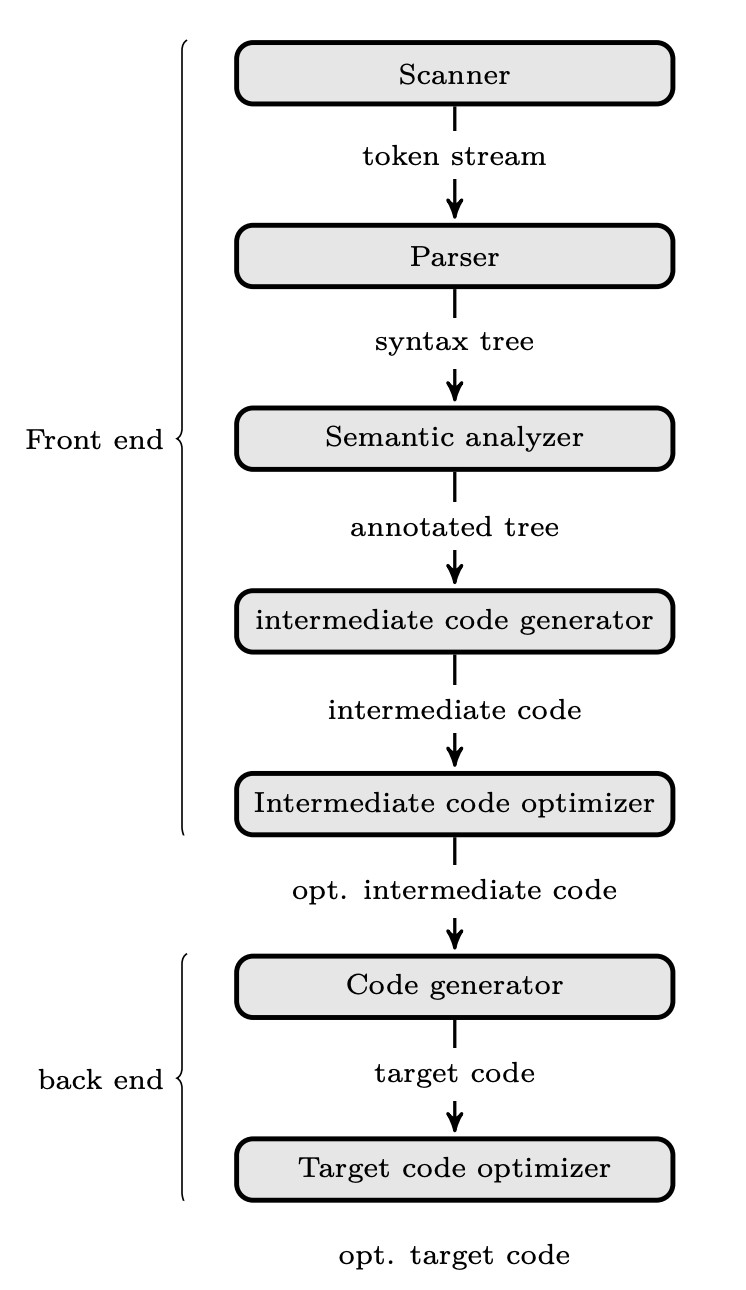
\includegraphics[scale=0.35]{assets/compilerOutline.png}
    \caption{The phases of a typical compiler.}
    \label{fig:compilerOutline}
\end{figure}

\subsection{Source-to-Source Compilers}

A transpiler, formally \textbf{source-to-source compiler}, is a tool that converts input source code to output source code, whilst maintaining a similar abstraction level~\cite{whatIsATranspiler}. The first transpiler to our knowledge was developed in 1978 by Intel, with the aim of translating Assembly source code from an 8080/8085 processor to an 8086 processor~\cite{theFirstTranspiler}. \\

JavaScript, the world's most commonly used programming language~\cite{javaScriptIsCommon}, has a rich history of transpilation. As a language in constant development, it faces an issue where not all browsers are always compatible with its newest features. Babel is a transpiler that converts modern JavaScript into a backwards compatible version.~\footnote{Babel can be accessed on \url{https://babeljs.io}} According to Nicolini et al., without a transpiler almost 14\% of web users risk facing a JavaScript bug when accessing a website with new JavaScript features~\cite{DBLP:journals/software/NicoliniHF24}. \\

Not only JavaScript can be transpiled to JavaScript. In fact, the list of other programming languages and tools that can be transpiled to JavaScript is so extensive that it could likely be a thesis topic of its own.~\footnote{This overview \url{https://gist.github.com/matthiasak/c3c9c40d0f98ca91def1} provides a list of 320 languages and tools that compile to JavaScript.} However, we can bring forward some notable exambles. \\

Contrary to JavaScript, TypeScript is structurally typed. TypeScript is syntactically a superset of JavaScript, adding a layer of static typing. The primary purpose of these types is to enhance the development experience by catching potential errors during compilation, as well as making the code more maintainable. However, before the code is run, TypeScript is transpiled into plain JavaScript, and the types are stripped away~\cite{TypeScript}. \\

AlaSQL is an open-source SQL database for JavaScript~\cite{alaSQL}. It lets us write SQL within a JavaScript context, i.e. creating tables and performing CRUD operations. \Cref{JavaScript AlaSQL.} shows how we can create a table, populate it with a a few italian football teams, before selecting the ones with enough points to our liking. \\

\begin{lstlisting}[caption={JavaScript code to create, populate and select a table with AlaSQL.}, captionpos=b, label={JavaScript AlaSQL.}]
alasql("CREATE TABLE
        teams (name string, points number)");

alasql("INSERT INTO teams
        VALUES ('SSC Napoli', 49),
               ('Salernitana', 15),
               ('Atalanta', 51)");

const topHalf = alasql("SELECT *
                    FROM teams
                    WHERE points < 40
                    ORDER BY points
                    DESC");
\end{lstlisting}

Despite all the commands being written in SQL, the selected table will have a JavaScript value, as seen in \Cref{The value of topHalf} \\

\begin{lstlisting}[caption={The value of topHalf from \Cref{JavaScript AlaSQL.}}, captionpos=b, label={The value of topHalf}]
[
    {
        "name": "Atalanta",
        "points": 51
    },
    {
        "name": "SSC Napoli",
        "points": 49
    }
]
\end{lstlisting}

JavaScript is practically the only Turing-complete programming language that can be used across browsers for web development. Rather than reinventing the wheel, developers have created transpilers to convert programs in their favourite languages to JavaScript. This allows them to write code in their preferred languages, also for web development. Notable examples inlcude GopherJS, Scala.js and Opal, which transpile Go, Scala and Ruby, respectively, to JavaScript. \\

Transpilation is not exclusive to JavaScript, however. It is a common practice in many other programming languages that must interact with or be portable across diverse systems. For instance, the Haskell compiler GHC (Glasgow Haskell Compiler) used to convert the code to C rather than direct native code generation. This enabled Haskell to run on any platform with a C compiler. It also benefitted directly from others' improvements in C code generation~\cite{HaskellToC}. \\

Another example is a transpiler presented by Lunnikiv et. al, where Python is converted to Rust as an intermediate source code step~\cite{PythonToRust}. The paper shows how pre-existing Python implementations that depend on optimised libraries can be semi-automatically transpiled to Rust. This way, the user can keep writing Python whilst simultaneously basking in the glow of Rust's performance optimisation.

\subsection{Parsers and Code Generators}

We mentioned that the frontend of a compiler is tasked with reading source code, and --- given that it is syntactically correct --- building an intermediate representation. The backend of a compiler is tasked with converting that intermediate representation into target code. \\

Having in-depth knowledge about the entire pipeline of a compiler is not necessary to understand the key points of this thesis. Nevertheless, two important aspects of a compiler that \textit{will} be central focus points, are parsers and code generators. Parsers and code generators play a vital role also in a transpiler. In fact, they are all we really need to build a simple transpiler. When the parser has converted the source code to an intermediate representation, the code generator can convert that intermediate representation into a target program. \\

Technically, the parser and the code generator are completely independent from one another. The only thing they must have in common is the ability to read or write the same intermediate representation. There are several advantages to this, like flexibility and modularity. If we want our transpiler to read or write another language, we can just create an additional parser or code generator. When we add a parser, we do not have to do any changes to our code generator, and vice versa, because they work on the same intermediate representation, independent of how the source- and target programs look like. \\

An example of this in practice is the programming language \textbf{Derw}, an ML language mainly inspired by Elm~\cite{derw}. It comes with a single parser (for the Derw language), but multiple code generators (referred to as just generators) which target JavaScript, TypeScript, Elm as well as English and Derw itself. As it is open sourced, anyone can fork the repository and add their own code generator, if they so desire. \\

\Cref{LTE in Derw} shows how expressions like \texttt{6 $<=$ 8} are converted. The token \texttt{lessThanOrEqual} has a left- and right pointer, corresponding to the respective integers. These are extracted, and put on each side of the string \texttt{is less than or equal to}.~\footnote{The entire English code generator is located at \url{https://github.com/eeue56/derw/blob/main/src/generators/English.derw}} \\

\begin{lstlisting}[caption={The function that converts a \texttt{Less than or equal}-expression in Derw to English.}, captionpos=b, label={LTE in Derw}]
generateLessThanOrEqual: LessThanOrEqual -> string
generateLessThanOrEqual lessThanOrEqual =
    let
        left: string
        left =
            generateExpression lessThanOrEqual.left

        right: string
        right =
            generateExpression lessThanOrEqual.right
    in
        `$\textdollar${left} is less than or equal to $\textdollar${right}`
\end{lstlisting}

Another example is \textbf{Pandoc}, which is software that converts between different markdown formats~\cite{whatIsPandoc}. It includes a Haskell library, as well as a command-line program. It is able to convert documents from 45 source formats to 63 target formats.~\footnote{See the entire list at \url{https://hackage.haskell.org/package/pandoc}} Additionally, Pandoc is able to convert documents in LaTeX, Groff ms and HTML into PDFs. \\

At its core, Pandoc is really just a specification of Haskell data types. A Pandoc document has the type \texttt{Pandoc Meta [Block]}. The first attribute is \texttt{Meta}, a document's metadata like its title, its author(s), the date it was written and more. The second attribute is a list of \texttt{Block}. A block is a more intricate data type, shown in its entirety in \Cref{Block data type in Pandoc}. \\

\begin{lstlisting}[caption={The \texttt{Block} data type of Pandocs native representation.}, captionpos=b, label={Block data type in Pandoc}]
Plain [Inline]
Para [Inline]
LineBlock [[Inline]]
CodeBlock Attr String
RawBlock Format String
BlockQuote [Block]
OrderedList ListAttributes [[Block]]
BulletList [[Block]]
DefinitionList [([Inline], [[Block]])]
Header Int Attr [Inline]
HorizontalRule
Table [Inline] [Alignment] [Double] [TableCell] [[TableCell]]
Div Attr [Block]
Null
\end{lstlisting}

The modular design of Pandoc means that adding an input format only requires the program to convert \textit{to} this native representation, whilst an output format only needs to convert \textit{from} it. This is much like parsers and code generators of compilers, but as they are much less intricate, the Pandoc documentation refers to them simply as \texttt{readers} and \texttt{writers}. Throughout this thesis, the words \texttt{writer} and \texttt{code generator} will be used interchangeably.~\footnote{In reality, traditional code generators do much more than directly translating data types to a target program. In the context of this thesis, however, code generators will not be asked to do much more. This is also a way to acknowledge that the writers we ultimately construct are not fully fledged code generators like one might see in compilers.} \\

Though it must be said, Pandoc cannot always ensure a completely lossless conversion. As the native representation is less expressive than many of the formats it converts between, details are bound to get lost on the way. For instance, LaTeX is a notoriously rich format, much more so than many of its companions in the Pandoc dynasty. However, Pandoc is an excellent interpreter of lightweight markup languages like Markdown, which are more \textit{neutural} by design~\cite{whatIsPandoc}. \\

An example of conversion with Pandoc is provided in \Cref{A Markdown program converted to LaTeX with Pandoc.}. The input format is Markdown, and the output format is LaTeX. \Cref{internalPandoc} shows the intermediate, native representation in Haskell. Meta contains title and date, while the list entries in Block are of type Header and Para. \\

\begin{figure}[ht]
\centering
\begin{subfigure}{.6\textwidth}
  \centering
  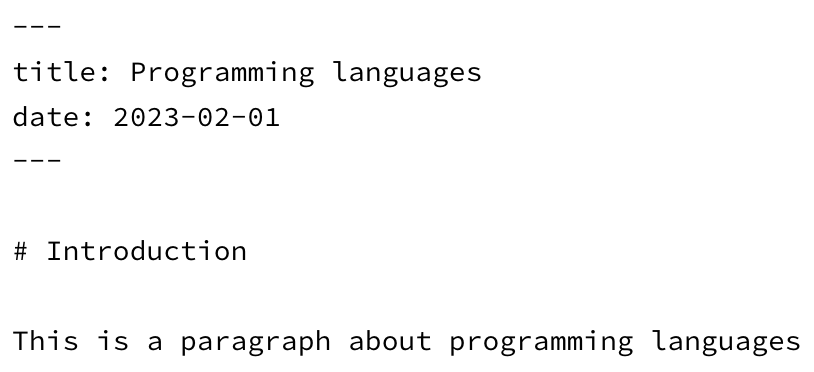
\includegraphics[width=1\linewidth]{assets/pandocMD.png}
  \caption{A Markdown program.}
  \label{markdownProgram}
\end{subfigure}
\begin{subfigure}{.6\textwidth}
  \centering
  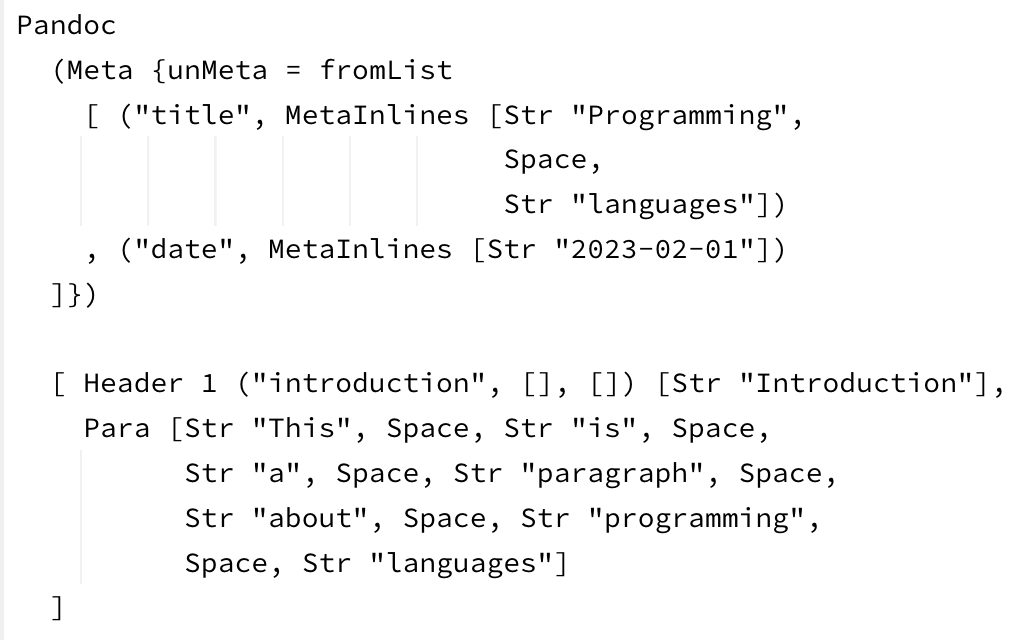
\includegraphics[width=1\linewidth]{assets/pandocHASKELL.png}
  \caption{The internal Pandoc AST of \Cref{markdownProgram}.}
  \label{internalPandoc}
\end{subfigure}
\begin{subfigure}{.6\textwidth}
  \centering
  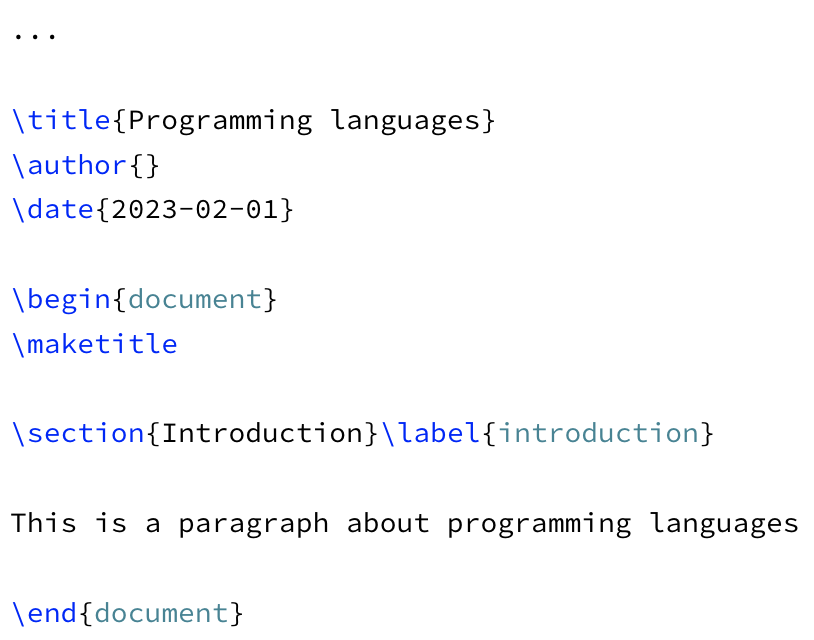
\includegraphics[width=1\linewidth]{assets/pandocLATEX.png}
  \caption{A LaTeX program, built from the AST in \Cref{internalPandoc}.}
  \label{latexResultOfPandoc}
\end{subfigure}

\caption{A Markdown program converted to LaTeX with Pandoc.}
\label{A Markdown program converted to LaTeX with Pandoc.}
\end{figure}
